\documentclass{wptemp}
\usepackage{adjustbox}
\usepackage{dcolumn}    % aligning decimals
    \newcolumntype{d}[1]{D{.}{.}{#1}}
% *****************************************************************
% Estout LaTeX wrapper
% *****************************************************************

\usepackage{lscape}
\usepackage{threeparttablex}
\usepackage{longtable}

%%Original code developed by Jörg Weber: see
%% https://www.jwe.cc/2012/03/stata-latex-tables-estout/
%% and
%% https://www.jwe.cc/blog/

% Redefine figure and table counters to use Arabic numerals
\renewcommand{\thefigure}{\arabic{figure}}
\renewcommand{\thetable}{\arabic{table}}


\let\estinput=\input % define a new input command so that we can still flatten the document

\newcommand{\estwide}[3]{
		\vspace{.75ex}{
			%\textsymbols% Note the added command here
			\begin{tabular*}
			{\textwidth}{@{\hskip\tabcolsep\extracolsep\fill}l*{#2}{#3}}
			\toprule
			\estinput{#1}
			\bottomrule
			\addlinespace[.75ex]
			\end{tabular*}
			}
		}	

\newcommand{\estauto}[3]{
		\vspace{.75ex}{
			%\textsymbols% Note the added command here
			\begin{tabular}{l*{#2}{#3}}
			\toprule
			\estinput{#1}
			\bottomrule
			\addlinespace[.75ex]
			\end{tabular}
			}
		}

% Allow line breaks with \\ in specialcells
\newcommand{\specialcell}[2][c]{%
    \begin{tabular}[#1]{@{}c@{}}#2\end{tabular}
}

\newcommand{\sym}[1]{\rlap{#1}}% Thanks David Carlisle


%%%%%%%%%%% End of wrapper %%%%%%%%%%%%%%%%%%%%%
    
%%%%%%%%%%% TiKz %%%%%%%%%%%%%%%%%%%%%
\usepackage{tikz}
\usetikzlibrary{shapes.geometric, arrows}

\tikzstyle{startstop} = [rectangle, rounded corners, minimum width=3cm, minimum height=1cm,text centered, draw=black, fill=red!30]

\tikzstyle{io} = [trapezium, trapezium left angle=70, trapezium right angle=110, minimum width=3cm, minimum height=1cm, text centered, text width =5cm, draw=black, fill=blue!30]

\tikzstyle{process} = [rectangle, minimum width=3cm, minimum height=1cm, text centered, text width =5cm, draw=black, fill=orange!30]

\tikzstyle{decision} = [diamond, minimum width=3cm, minimum height=1cm, text centered, draw=black, fill=green!30]

\tikzstyle{arrow} = [thick,->,>=stealth]

\begin{document}

\linespread{1}{\title{{\fontfamily{ptm}\selectfont{\Large{\MakeUppercase{The Impact of Hispanic Last Names and Identity on Labor Market Outcomes}}}}
\thanks{I thank Professors Willa Friedman, Chinhui Juhn, Vikram Maheshri, and Yona Rubinstein for their support and advice. I also thank Aimee Chin, Steven Craig, German Cubas, Elaine Liu, Fan Wang, and the participants of the Applied Microeconomics Workshop at the University of Houston.}
}}
	\author{{\fontfamily{pbk}\selectfont\large{\textsc{Hussain Hadah}}\thanks{Department of Economics, Tulane University, 6823 St. Charles Ave., New Orleans, LA 70118, United States, (phone: +1-602-393-8077, e-mail: \email{hhadah@tulane.edu}). Competing interests: The author declares none.}}}
	\date{\fontfamily{pbk}\selectfont\normalsize{\textsc{\today}}}
	\maketitle

\begin{center}
\href{https://hhadah.github.io/hispanic-last-names/my_paper/Hadah-last-names.pdf}{\textcolor{green!15!black!30!blue}{\footnotesize{\textsc{Click Here to Get the Most Updated Version}}}}
\end{center}
	
\pagenumbering{arabic}

\begin{abstract} 
In this paper, I study discrimination against Hispanics in the labor market. I compare the children of inter-ethnic marriages to study the impact of having a Hispanic last name. While males born to Hispanic father-White mothers earn 6 percentage points less than those born to White father-Hispanic mothers, the gap could be completely explained by educational differences. I also study the effect of identifying as Hispanic on earnings. I find that men with a Spanish-sounding last name who identify as Hispanic earn significantly less than those who do not identify as Hispanic, but the gap could also be explained by educational differences.

\keywords{Economics of Minorities, Race, and Immigrants; Discrimination and Prejudice.}
\JEL{J71; J64}

\end{abstract}

\pagebreak
\section{Introduction}\label{sec:intro}

A large literature documents substantial earnings gaps across race and ethnicity \citep{bayer2018divergent, charles2008prejudice, card1992school, fryer2004causes, rubinstein2014pride, bertrand2004emily, juhn1991accounting}. Hispanics constitute a large and growing portion of the population in the United States. As the number of Hispanics increases, determining whether ethnic discrimination affects their labor market outcomes becomes increasingly crucial \citep{chettyUnitedStatesStill2014, chettyEffectsExposureBetter2016,chettyFadingAmericanDream2017,abramitzkyImmigrantsAssimilateMore2020a, abramitzkyNationImmigrantsAssimilation2014,abramitzkyCulturalAssimilationAge2016,chettyWhereLandOpportunity2014}. Thus, it is important to understand whether a person's ethnicity affects their labor market outcomes. Assimilation and mobility are crucial because they reflect how well Hispanics can integrate into society and move up the socioeconomic ladder.

In this paper, I answer the following questions. Does having a Hispanic last name affect labor market outcomes? What is the effect of identifying as Hispanic on earnings? Moreover, I aim to show that comparing Hispanic Whites to non-Hispanic Whites might create an artificially higher earnings gap since the two groups differ on many observable characteristics.\footnote{By identifying as Hispanic, I refer to individuals who self-report their ethnicity as Hispanic on surveys or other data collection instruments.} \footnote{Observable characteristics refer to factors that can be measured and quantified, such as education level, work experience, and immigration status.} Others have attempted to compare how native-born White Hispanics fare to non-Hispanic Whites and foreign-born Hispanics. In \citet{antman2020ethnic,antmanEthnicAttritionObserved2016,antmanEthnicAttritionObserved2016a,antmanEthnicAttritionAssimilation2020}, the authors compare the health and educational outcomes of Hispanic Whites to non-Hispanic Whites and native-born Hispanics to foreign-born Hispanics. They find gaps in education and health between Hispanics and Whites. They also find that native-born Hispanics are more likely than their foreign-born counterparts to report poor health. \citet{davilaChangesRelativeEarnings2008} documents many gaps in labor market outcomes between Hispanics and Whites. They attribute a big part of this gap to differences in education, experience, immigration status, and regional differences. 

The US population is growing in diversity. The proportion of non-Whites has increased by more than 10 percentage points from 13 percent in 1995 to 23 percent in 2019. The number of Hispanics has grown by 9 percentage points from 9 percent in 1995 to 16 percent in 2019.\footnote{The portion of non-Whites and Hispanics is calculated using the Current Population Survey (CPS).} Native-born White Hispanic men earn 21\% less than White men, although a substantial portion of the earnings gap is due to educational differences between Hispanics and Whites \citep{duncan2006hispanics, duncan2018identifying, duncan2018socioeconomic}. Some of the earnings differences may also be due to discrimination which will have negative consequences. For example, discrimination against Hispanics can lead to reduced job opportunities, lower wages, and hinder assimilation. In this paper, I examine the role of having a Hispanic last name and identifying as Hispanic on labor market outcomes. 

Identifying discrimination is difficult because of factors that affect labor market outcomes that are unobservable to economists---such as unobserved skills. One strategy used by researchers is audit or resume studies. \citet{bertrand2004emily} conducted an audit study where identical resumes were sent to employers with White and Black-sounding names. This approach, however, has its drawbacks. Audit studies only observe callbacks, not wages. 

This study utilizes a method developed by \citet{rubinstein2014pride}. I compare children from inter-ethnic marriages. More precisely, I compare children of Hispanic fathers and White mothers (henceforth HW) to children of White fathers and Hispanic mothers (henceforth  WH). This approach stems from the fact that marriages are not random. Couples match on several observable characteristics like income, schooling, socio-economic background, etc. \citep{averettBetterWorseRelationship2008, averettEconomicRealityBeauty1996, beckerTheoryMarriagePart1973, beckerTheoryMarriagePart1974, beckerTreatiseFamily1993, browningCollectiveUnitaryModels2006, chiapporiFatterAttractionAnthropometric2012}. Children of HW and WH marriages have more similar observable characteristics than children of endogamous/homogamous marriages--- i.e., White fathers-White mothers and Hispanic fathers-Hispanic mothers. Moreover, children from a Hispanic father and White mother household will have a Hispanic last name from their fathers, enabling the investigation of how ethnic signals, such as having a Hispanic last name, affect annual log earnings.

Using the Current Population Survey (CPS) from 1994 to 2019 and the 1960 to 2000 US censuses, I estimate the effect of having a Hispanic last name on labor market outcomes. In other words, I approximate the variation in labor market perception of ethnic signals, in this case having a Hispanic last name, on annual log earnings. I also study the effect of identifying as Hispanic on labor market outcomes. 

I find that while men born to Hispanic father-White mothers earn less than men born to White father-Hispanic mothers, this gap is entirely explained by educational differences. Thus, I do not find a significant effect of having a Hispanic last name. Finally, I find that men identifying as Hispanic earn significantly less than those who do not, even when I control for ancestry and education.

% Inter-ethnic children with a White father, and thus having a non-Hispanic last name, earn 14\% less than children of endogamous White parents. Inter-ethnic children with a Hispanic father, and thus having a Hispanic last name, earn 20\% less than children of endogamous White parents. Endogamous children with Hispanic parents earn 24\% less than children of endogamous White parents. A big part of the gaps could be explained by education. Inter-ethnic children with a White father and identify as Hispanic, and thus having a non-Hispanic last name, earn 14\% less than children of endogamous White parents. Inter-ethnic children with a Hispanic father and identify as Hispanic, and thus having a Hispanic last name, earn 18\% less than children of endogamous White parents. Endogamous children with Hispanic parents and identify as Hispanic earn 10\% less than children of endogamous White parents.


Previous studies have also used names as a proxy for race and ethnicity \citep{fryer2004causes, rubinstein2014pride, bertrand2004emily}. \citet{fryer2004causes} point out that names can be a predictor of a person's race. Specifically, they provide a rising pattern among Blacks having different names than Whites. They did, however, find that having a Black name, after controlling for the home environment at birth, does not affect their labor market outcomes. \citet{rubinstein2014pride} compared the children of mixed marriages between Sephardic and Ashkenazi Jews in Israel.\footnote{Ashkenazi and Sephardic are two distinct Jewish ethnic groups.} They found that workers with Sephardic last names earn substantially less than those with Ashkenazi last names. \citet{bertrand2004emily} conducted an audit study by sending employers identical resumes that differ in the ethnic and racial signal of a name (Black sounding name versus a White sounding one). They found that resumes with Black-sounding names received substantially fewer callbacks than their White counterparts. 

The rest of the paper is organized as follows. Section \ref{sec:data} provides an overview of the data and summary statistics of the sample. Section \ref{sec:emp_model} introduces the empirical framework. I report the results in section \ref{sec:results}. Finally, I offer a brief conclusion in section \ref{sec:con1}.

\section{Data}\label{sec:data}

I use two datasets:  the Integrated Public Use Microdata Series (IPUMS) Current Population Survey (CPS) Annual Social and Economic (ASEC) \citep{cps2019} and the 1960 to 2000 US censuses \citep{acs2019}. 

I use the CPS data set to study the effect of having a Hispanic last name on a person's labor market outcomes. I take advantage of the fact that the CPS asks parents' place of birth, ethnicity, and race. The data spans the period between 1994--- the earliest sample to ask about a parent's place of birth--- to 2019. Moreover, since the CPS does not provide data on parents' characteristics, essential to determine the family background, I use the census to construct synthetic parents. The census offers a larger sample of potential parents. Similar to the CPS, the 1960 to 2000 censuses ask about the person's place of birth and the individual's race and ethnicity. I employ this information to construct "synthetic parents" using a method developed by \citet{rubinstein2014pride}. I construct the synthetic parents by linking husbands and wives in the census data to each other. I assume that parents have children between the ages of 25 and 40. I then link these synthetic parents using the birth year of child, and place of birth of parents to the year of birth of the "children" and the palce of birth of parents in the CPS sample.

\subsection{Children of the four parental types}

I use the CPS for my primary analysis of the effect of having a Hispanic last name on earnings. I restrict my sample to Whites, United States-born citizens aged 25 to 40 and born between 1960 to 2000. Taking advantage of data on parents' place of birth, I divide the sample into four groups depending on their parent's ethnicity. Mothers or fathers are Hispanic if they were born in a Spanish-speaking country and Puerto Rico, and White if they were born in the United States.\footnote{The list of Spanish Speaking countries include: Argentina, Bolivia, Chile, Colombia, Costa Rica, Cuba, Dominican Republic, Ecuador, El Salvador, Guatemala, Equatorial Guinea, Honduras, Mexico, Nicaragua, Panama, Paraguay, Peru, Spain, Uruguay, Venezuela.} Therefore, an observation can be the product of four types of parents: 
\begin{enumerate}
\item White father and White mother (hereafter WW) 
\item White father and Hispanic mother (hereafter WH)
\item Hispanic father and White mother (hereafter HW)
\item Hispanic father and Hispanic mother (hereafter HH).
\end{enumerate}

The distribution of the four types of children is presented in figure \ref{fig:dist} and table \ref{tab:mat1}. The majority of the sample (95.96\%) is WW children. The second biggest group is HH, which constitutes 2.69\% of the sample. Inter-ethnic children, WH and HW, make up 1.35\% of the sample with 90,325 observations. Even though WH and HW are only 1.35\% of the sample, I have plenty of observations to carry out an analysis. The summary statistics for the children of the four types of marriages are presented in table \ref{tab:c&p1}. Children of WW marriages (column 1) do better on every measure while children of HH parents (column 4) do worse than other children on every measure. 

On the one hand, WW children are more educated, with approximately 14 years of education for men and women. WW children have an unemployment rate of 4\% for men and women. They have log hourly earnings of 2.51 for men and 2.32 for women. Also, their annual log earnings are 10.29 for men and 9.43 for women.

On the other hand, children of HH marriages have an average of 12.9 and 13.24 years of education for men and women, respectively. HH men and women have an unemployment rate of 7\% and 6\%. Their annual log earnings are 10.01 and 9.53 for men and women, respectively. 

Inter-ethnic children, WH and HW, have lower educational attainment and income than WW children, but they are better than HH children. Also, WH and HW are comparable, unlike WW and HH children. These two groups are important to the analysis. Children of HW are going to be the treatment group. HW children have a Hispanic father with a Hispanic last names. At the same time, the WH children have White fathers with a non-Hispanic, or White, last names. Summary statistics of these two groups, table \ref{tab:c&p1} columns (2) and (3) can show that they are different from the children of non-inter-ethnic marriages. 


WH children have an average of 13.58 and 13.79 years of education for men and women. The unemployment rate for men and women is 5\%. HW men and women obtained 13.22 and 13.42 years of schooling. Men's unemployment rate is 7\% and women's 6\%.

In panel C of table \ref{tab:c&p1}, I present the rates at which members of each group self-identify as Hispanic. \footnote{Hispanic self-identification is observed when an individual notes that they are Hispanic on the CPS questionnaire} The vast majority of HH children, 96\% for men and 97\% for women, identify as Hispanic. There is considerable attrition in Hispanic identification of inter-ethnic children. Among WH children, 74\% of men and 78\% of women identify as Hispanic. Among HW children, 83\% of men and 82\% of women identify as Hispanic. These results align with the findings of a substantial body of literature that noted this attrition among children of immigrants, especially those coming from inter-ethnic marriages \citep{duncan2017complexity, duncan2018identifying, duncan2020new, antman2020ethnic}. Finally, a small portion of WW children, 4\% of men and 5\% of women, identified as Hispanic. These 5\% of WW children are most likely third generation--- or higher--- children of immigrants. For my analysis, I dropped the WW observations who identify as Hispanic when I compare with non-Hispanic Whites.

In columns (5) and (6), I calculate the differences in means between HH-WW (column 5) and HW-WH (column 6). Overall, HH children do worse than WW children. HH has one year less of education compared to WW, and are 2 percentage points more likely to be unemployed. HH men earn 9\% less than WW men, and HH women make 2\% less than WW women. Therefore, these two groups, HH and WW, are different on many observable qualities.

The differentials between WH and HW are not as severe as the ones between HH and WW. HW children are still worse off than WH but are much better than HH. HW men attain 0.36 fewer years of education than WH men. HW women achieve 0.37 fewer years of schooling than WH women. HW children are 1 percentage points more likely to be unemployed. HW men earn 1\% less annual earnings as WH men, and HW women earn 3\% less. These differences show that HW and WH children are different from children of endogamous/homogamous marriages and, thus, are more comparable.

In table \ref{tab:c&p2}, I present the summary statistics for the four types and limit the sample to those that only identify as Hispanic.\footnote{Limiting the sample to those who identify as Hispanic only affects WH, HW, and HH. Members of the WW group are not affected by this restriction.} The same pattern discussed above between HH--WW and HW--WH persists. The one difference is that those who identify as Hispanic do slightly worse.
 
\subsection{Synthetic parents}

Using the 1960 to 2000 censuses, I constructed a data set of synthetic parents. The sample includes married White men and women. Even though the census asks a person whether they are Hispanic or not, I took advantage of the questions on place of birth to create a proxy for ethnicity. I consider a Hispanic person as White and born in a Spanish-speaking country. Consequently, Whites in the sample are people who are White and native-born. Using the information provided in the census, I can link husbands and wives with each other. I assume that parents have children between the ages of 25 and 40. Therefore, my sample consists of married White men and women with children that were born in the 1920 to 1975 cohorts\footnote{The construction of "synthetic parents" follows the method used by \citet{rubinstein2014pride}.}.

I show the distribution of the four types of couples in table \ref{tab:mat2}. White husbands and White wives (WW) make up the majority of couples in the sample, 96\% (5,141,737 couples). Hispanic husbands and wives (HH) are the second largest group making up 2\% (119,749 couples) of all couples. White husbands and Hispanic wives (WH) couples are less 1\% (33,097 couples) of the sample and Hispanic husbands and White wives (HW) are also 1\% (37,847 couples). 


I present the summary statistics of the four types of synthetic parents in table \ref{tab:synth}. WW couples have higher education, 12.75 years for husbands and 12.47 for wives. As a household, WW couples have 25.22 years of schooling. Additionally, the log total family income for a WW household is 10.72 and have 3.77 children. Husbands in HH marriages have 8.64 years of education, while women have 8.49 years of schooling. As a household, HH couples have 17.13 years of education, log total family income of 10.27, and have 4.23 children.

WH husbands have 11.77 years of education, while wives have an average of 10.40 years. WH household attained a total of 22.17 years of schooling in total, a log total family income of 10.55, and 3.98 children. HW husbands and wives obtained 10.25 and 11.11 years of education, respectively. HW household attained a total of 21.36 years of schooling in total, a log total family income of 10.46, and 4.15 children.


In columns 5 and 6 of table \ref{tab:synth}, I report the differences in means between HH-WW households and HW-WH households. An HH Hispanic husband attained 4.11 fewer years of education than a WW husband. While an HH wife acquired 3.98 fewer years of schooling than a White WW wife. The total educational difference between HH and WW households equals 8.09 years of education. The educational differences between HW and WH are less severe than those between HH and WW. A Hispanic husband in intermarriage attained 1.52 fewer years of schooling than a White husband in intermarriage. A White wife in intermarriage attained 0.70 years of education, more than a Hispanic wife in intermarriage. The difference in total years of education between HW and WH households is 0.81, which is an 90\% decrease from the HH--WW gap. The total family income of an HH household is 45\% lower than a WW household, while the total family income of an HW household is 10\% lower than a WH household. These differences show that couples that intermarry are better and different than those that do not.


%In table \ref{tab:p1} columns five and six, I provide the  HH-WW and HW-WH gaps. WW couples are more educated and earn more than HH couples. Also, WH husbands are more educated and earn more than HW husbands. In comparison, WH wives are more educated than HW wives. Even though White husbands in intermarriages are more educated and earn more than husbands in HW marriages, they are more comparable to each other than the non-intermarriage couples.

\section{Empirical Strategy}\label{sec:emp_model}

In this section, I present two empirical strategies. The first empirical strategy estimates the effect of having a Hispanic last name on annual log earnings. The second empirical strategy estimates the effect of identifying as Hispanic on log annual earnings.

The difference in means between Hispanics and non-Hispanic Whites could result from discrimination. It can also be caused by differences in innate abilities, skills, and parental investments. While controlling for observable skill measures, I compare children of inter-ethnic marriages, HW and WH. WH and HW children are more similar in characteristics but provide employers, and the labor market, with different signals.\footnote{WH and HW children are both half White, half Hispanic.} WH children will have a non-Hispanic last name, while HW children will have a Hispanic last name. This is a method developed by \citet{rubinstein2014pride}.

\subsection{Estimating the effect of having a Hispanic last name}

In this section I restrict the sample to WH and HW groups. Let $Y_{ist}$ be the annual log earnings of person $i$ in state $s$ at time $t$. $HW_{ist}$ is an indicator variables for the type of parents person $i$ has. $X_{ist}$ is a vector of controls that includes age and numbers of hours worked, $\gamma_{t}$ are year fixed effects, $\lambda_{s}$ are state fixed effects, and $\phi_{ist}$ represents the error term. The equation for this strategy is written as follows:
\begin{equation} \label{eq:1a}
Y_{ist} = \beta_{1} HW_{ist} + X_{ist} \pi + \gamma_{t} + \lambda_s + \phi_{ist}
\end{equation}

$\beta_{1}$ is the coefficient of interest in this specification. $\beta_{1}$ represents the earnings gaps between children of inter-ethnic marriages who have a Spanish-sounding last name versus a White last name. 

\subsection{Estimating the effect of identifying as Hispanic}

In this section, I will present an estimation strategy that would allow me to capture the effect of identifying as a Hispanic. 

\begin{equation} \label{eq:iden}
Y_{ist} = \beta_{1} HW_{ist} + \beta_{2} Hispanic_i + \beta_{3} HW_{ist} \cdot Hispanic_i + X_{ist} \pi + \gamma_{t} + \lambda_s + \phi_{ist}
\end{equation}

The coefficients of interest from equation \ref{eq:iden} are $\beta_{1}$, $\beta_{2}$ and $\beta_{3}$. The coefficients $\beta_{1}$ and $\beta_{3}$ capture the effects of Spanish-sounding last names for $HW_{ist}$ that identify as Hispanic \textit{versus} those who do not.

\section{Results}\label{sec:results}

In this section, I present the results from estimating the two specifications in equations \ref{eq:1a} and \ref{eq:iden}. The results are shown in tables \ref{tab:lastnamereg} and \ref{tab:identreg}. All estimations are done on a sample of White, native-born men between the ages of 25 and 40 employed for full-time full-year (FTFY) and are wage and salary workers.

I find that an inter-ethnic person with a Spanish-sounding last names earns less than an inter-ethnic who has a White last name. A person with a Spanish-sounding last name earns 5 percentage points less than a person with a White last name. In other words, by comparing inter-ethnic children, a person with a Hispanic last name earns 5 percentage points less than someone with a White last name. However, more than half of the earnings gaps could be explained by educational differences. When I control for education, the last name effect decreases to a statistically insignificant 2 percentage points earnings gap. I also find a significant earnings gap between those that identify as Hispanic. 

\subsection{The Effect of Having a Hispanic Last Name and Hispanic Identity on Labor Market Outcomes}

I provide the results to the estimation of equation \ref{eq:1a} in table \ref{tab:lastnamereg}. The sample in this analysis includes full-time, full-year, and wage and salary men, and I control for hours worked and age and include year fixed effects (FE). I also restrict the sample to children of HW and WH (omitted) parents. Column one in table \ref{tab:lastnamereg} is the results without controlling for education. Overall, an inter-ethnic with a Hispanic last name earns 6 percentage points less than an inter-ethnic with a White last name. This gap, however, could be entirely explained by educational differences. An inter-ethnic with a Hispanic last name earns 6 percentage points less than an inter-ethnic with a White last name, but the result is statistically insignificant.

I provide the results to the estimation of equation \ref{eq:iden} in table \ref{tab:identreg}. The sample in this analysis includes full-time, full-year, and wage and salary men, and I control for hours worked and age and include year fixed effects (FE). I also restrict the sample to children of HW and WH parents. The omitted group is children of WH parents that do not identify as Hispanic. Column one in table \ref{tab:identreg} is the results without controlling for education. An inter-ethnic $HW_{ist}$ that identifies as Hispanic \textit{versus} $HW_{ist}$ who do not---i.e. $HW_{ist} + HW_{ist} \cdot Hispanic_i$---earns 6 percentage points less than an inter-ethnic that does not, but the result could be entirely explained by educational differences.


\section{Conclusion}\label{sec:con1}

As the Hispanic population grows in the United States, studying discrimination against this group becomes increasingly important. In this paper, I examine discrimination against Hispanics in the labor market. More specifically, I examine the impact of Hispanic last names and Hispanic identification on annual log earnings. 

I compare the children of inter-ethnic marriages to study the labor market impact of having a Hispanic last name. When I compare the earnings of HW and WH children, which captures the effect of having a Hispanic last name, HW children earn  6 percentage points less than WH children. Thus, by comparing inter-ethnic children, a person with a Hispanic last name makes 6 percentage points less than someone with a White last name. When I control for education, the last name effect decreases to a statistically insignificant 2 percentage points earnings gap. Moreover, I estimate the effect of identifying as Hispanic and having a Hispanic last name. I find that an inter-ethnic child with a Hispanic last name and identifies as Hispanic earns 5 percentage points less that an inter-ethnic child with native sounding last name and identifies as Hispanic. 

While the earnings gap between children of inter-ethnic parents with and without a Hispanic last name disappears when controlling for education, it does not necessarily indicate the absence of discrimination. Education itself can be influenced by bias, potentially resulting in divergent outcomes. Consequently, further research is essential to comprehensively understand the earnings gaps between Hispanics and Whites.





% \nocite{*}
\pagebreak
\bibliography{HispanicDiscriminationMarriageMarket}
\newpage
\pagebreak
\begin{appendices}

\section{Figures}\label{appendix:figures}


% \begin{center}
% \begin{figure}[h!]
% \caption{Inter-racial marriages as a percent of all marriages \\
%  in the United States from 1995 to 2020.}
% 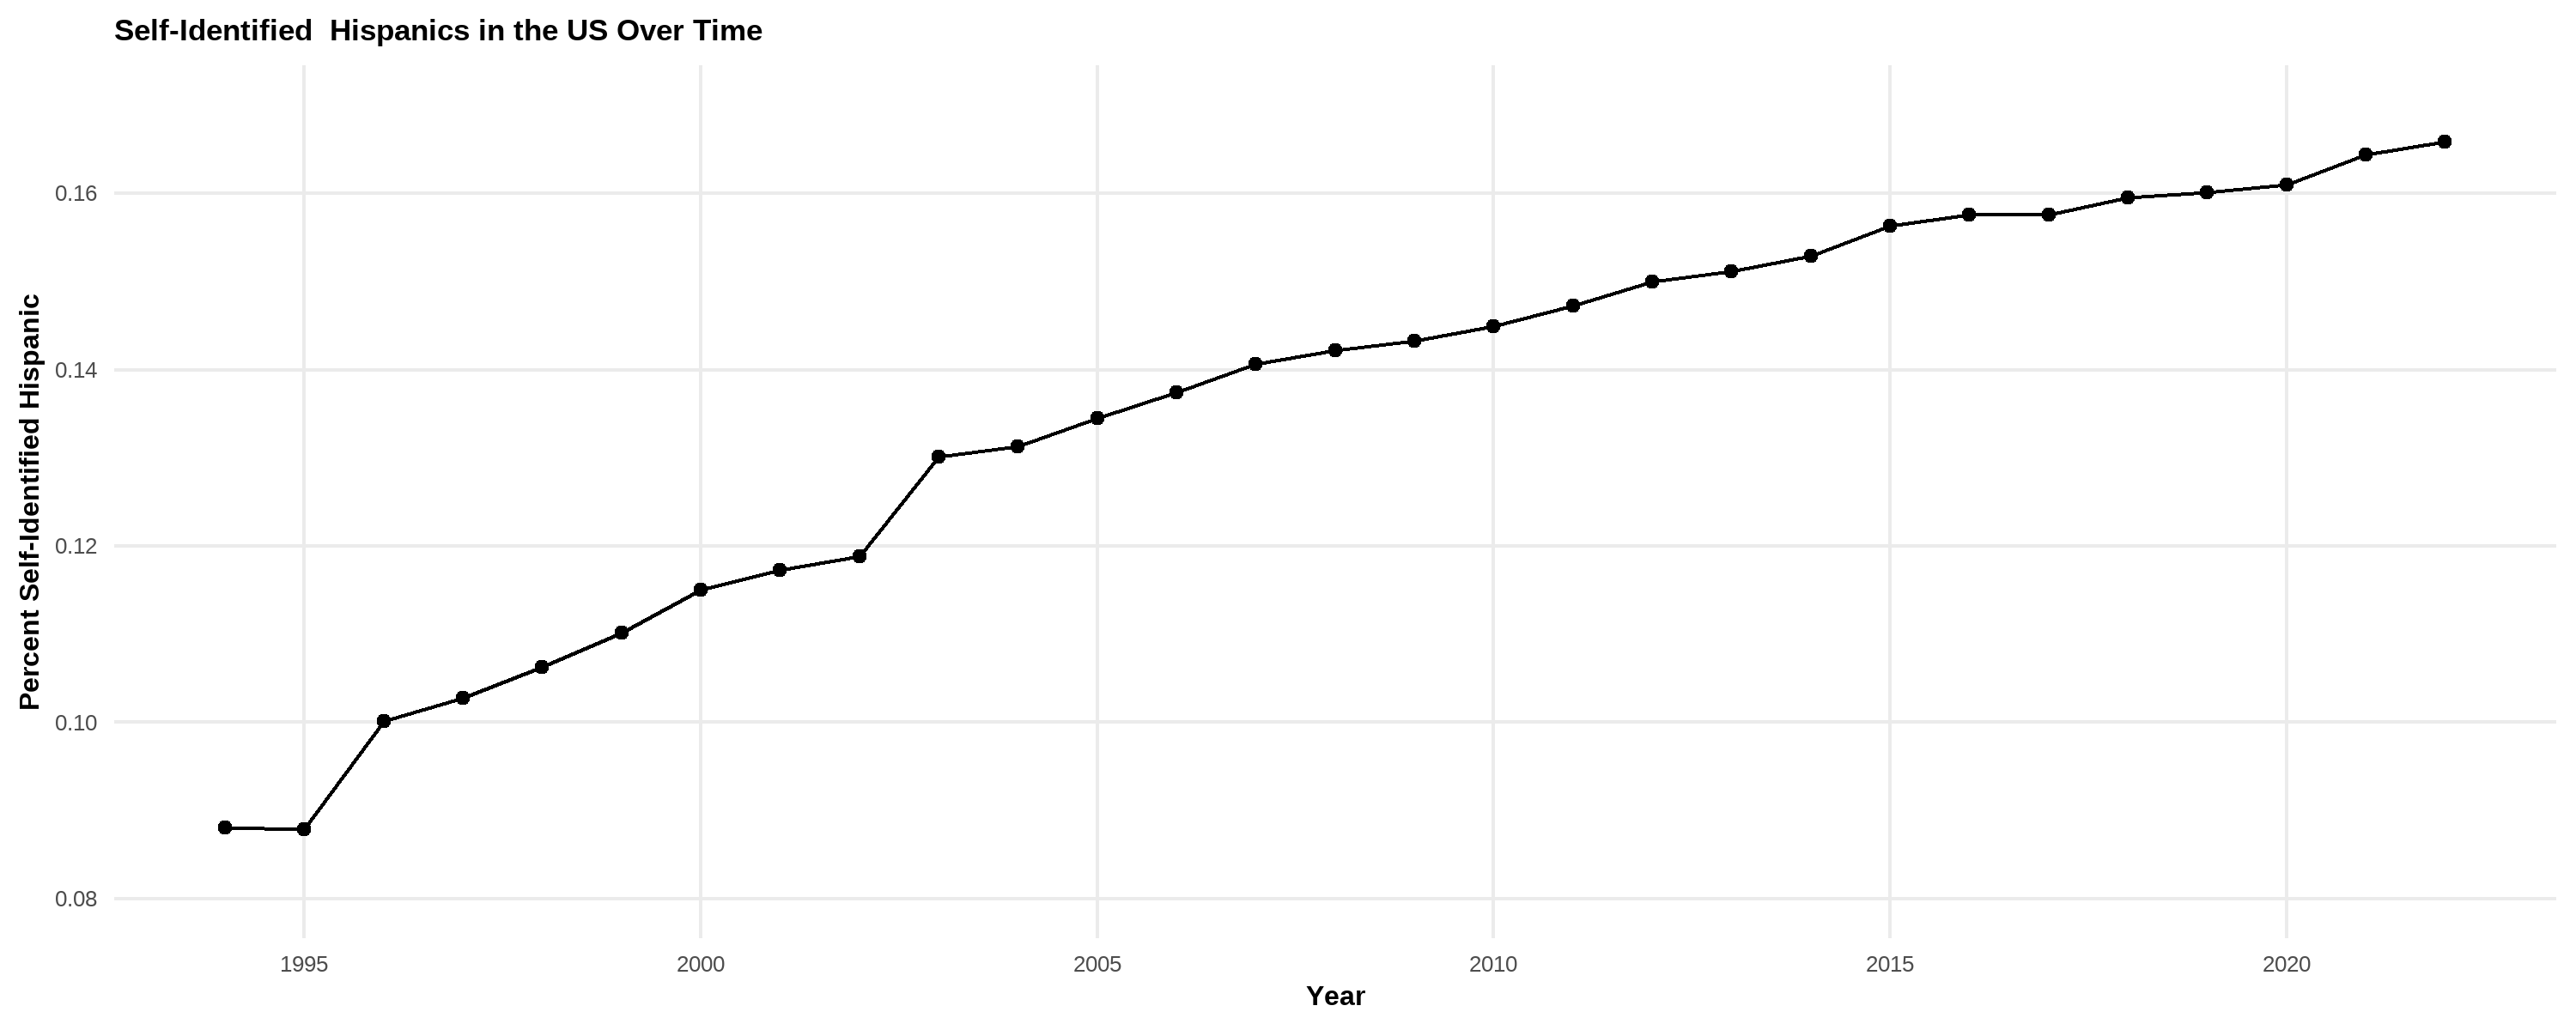
\includegraphics[width=\textwidth]{figures/Hispanics_all.png} 
% \label{fig:3}
% \end{figure}
% \end{center}

% \newpage

\begin{center}
\begin{figure}[h!]
\caption{Distribution of the four types of children.}
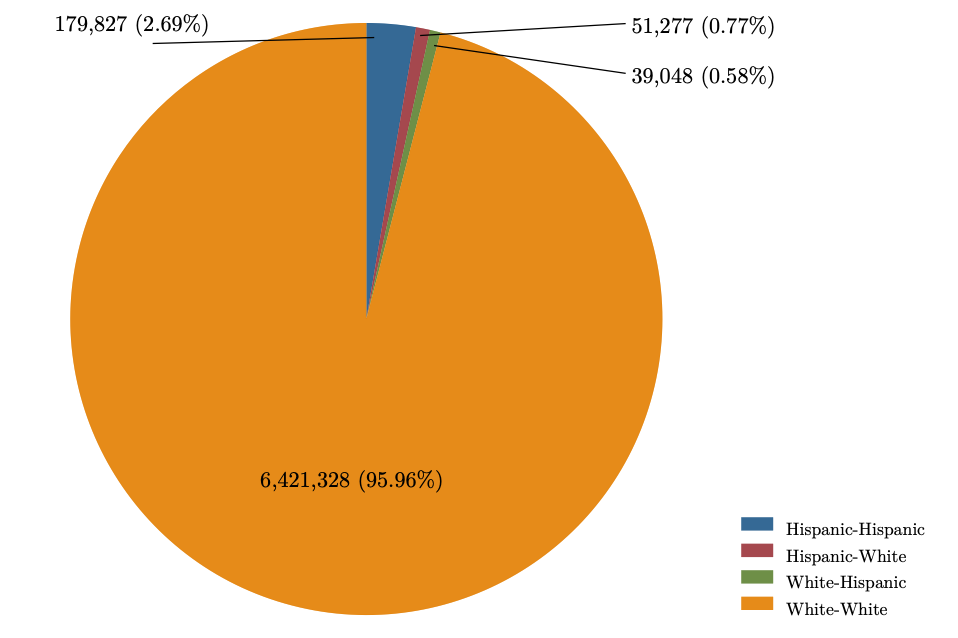
\includegraphics[width=\textwidth]{PirChart2.png} 
\label{fig:dist}
\end{figure}
\end{center}

% \newpage

% \begin{figure}[h!]
% \centering
% \caption{Chart explaining which synthetic parents and children and when we observe them.}
% \begin{tikzpicture}[node distance =2cm]
% \node (start) [startstop] {Synthetic Parents: Observed in 1960 to 2000. $25 \leq age \leq 40$, White, with kids};

% \node (pro1) [process, below of = start, yshift = -2cm] {Children: Observed between 1994 and 2019. Born between 1954 to 1999 and $25 \leq age \leq 40$};

% \draw [arrow] (start) -- (pro1);
% \end{tikzpicture}
% \label{flowchart1}
% \end{figure}

\newpage

\section{tables}\label{appendix:tables}

\begin{table}[t]
\tablefont
\caption{Number of Children by Parental Type \label{tab:mat1}}
%\resizebox{\linewidth}{!}{
\begin{threeparttable}
\begin{tabular}[t]{>{}lcccc}
\toprule
\multicolumn{1}{c}{ } & \multicolumn{4}{c}{Perental Type} \\
\cmidrule(l{3pt}r{3pt}){2-5}
  & \specialcell{White Father \\ White Mother} & \specialcell{White Father \\ Hispanic Mother} & \specialcell{Hispanic Father \\ White Mother} & \specialcell{Hispanic Father \\ Hispanic Mother}\\
\midrule
\textbf{\specialcell{Observations\\Share}} & \specialcell{6,421,328\\0.96} & \specialcell{39,048\\0.01} & \specialcell{51,277\\0.01} & \specialcell{179,827\\0.03}\\
\bottomrule
\end{tabular}
\begin{tablenotes}
\item[1] Source: Current Population Surveys (CPS) 1994-2019
\item[2] The sample includes Whites, who are married, and are between the ages 25 and 40. Ethnicity of a person's parents are identified by the parent's place of birth. A parent is Hispanic if she/he was born in a Spanish-speaking country. A parent is White if she/he was born in the United States.
\end{tablenotes}
\end{threeparttable}
%}
\end{table}


\newpage

\begin{table}[!h]

\caption{Couples' Type \label{tab:mat2}}
\centering
\resizebox{\linewidth}{!}{
\begin{threeparttable}
\begin{tabular}[t]{>{}lcccc}
\toprule
\multicolumn{1}{c}{ } & \multicolumn{4}{c}{Couples' Type} \\
\cmidrule(l{3pt}r{3pt}){2-5}
  & \specialcell{White Husband \\ White Wife} & \specialcell{White Husband \\ Hispanic Wife} & \specialcell{Hispanic Husband \\ White Wife} & \specialcell{Hispanic Husband \\ Hispanic Wife}\\
\midrule
\textbf{Observations} & \specialcell{1,286,731\\(0.97)} & \specialcell{7,178\\(0.01)} & \specialcell{7,606\\(0.01)} & \specialcell{20,911\\(0.02)}\\
\bottomrule
\end{tabular}
\begin{tablenotes}
\item[1] The data is restricted to people interviewed in 1970 and 1960 and also White and married. I identify the ethnicity of a person through their place of birth. A parent is Hispanic if they were born in a Spanish-speaking country. A parent is White if they were born in the United States.
\item[2] The table includes information on the proportion of the four types of synthetic parents that I have constructed.
\end{tablenotes}
\end{threeparttable}}
\end{table}


\newpage


\begin{landscape}
\begin{ThreePartTable}
\begin{TableNotes}
\item[1] Source: The 1960-2000 Census for synthetic parents, and 1994-2019 Current Population Surveys (CPS) for children's outcomes
\item[2] The data is restricted to native-born United States citizens who are also White and between the ages of 25 and 40. I identify the ethnicity of a person's parents through the parent's place of birth. A parent is Hispanic if they were born in a Spanish-speaking country. A parent is White if they were born in the United States.
\end{TableNotes}
\begin{longtable}[t]{>{\raggedright\arraybackslash}p{5cm}cccccc}
\caption{Summary statistics of children's outcomes using parent's place of birth \label{tab:c&p1}}\\
\toprule
\multicolumn{1}{c}{ } & \multicolumn{4}{c}{Father's and Mother's Ethnicities} & \multicolumn{2}{c}{Differences} \\
\cmidrule(l{3pt}r{3pt}){2-5} \cmidrule(l{3pt}r{3pt}){6-7}
Variables & \specialcell{White \\ White \\ (WW) \\ (1)} & \specialcell{White \\ Hispanic \\ (WH) \\ (2)} & \specialcell{Hispanic \\ White \\ (HW) \\ (3)} & \specialcell{Hispanic \\ Hispanic \\ (HH) \\ (4)} & \specialcell{HH - WW \\ (5)} & \specialcell{HW - WH \\ (6)}\\
\midrule
\endfirsthead
\caption[]{Summary statistics of children's outcomes using parent's place of birth  \textit{(continued)}}\\
\toprule
Variables & \specialcell{White \\ White \\ (WW) \\ (1)} & \specialcell{White \\ Hispanic \\ (WH) \\ (2)} & \specialcell{Hispanic \\ White \\ (HW) \\ (3)} & \specialcell{Hispanic \\ Hispanic \\ (HH) \\ (4)} & \specialcell{HH - WW \\ (5)} & \specialcell{HW - WH \\ (6)}\\
\midrule
\endhead
\midrule
\multicolumn{7}{r@{}}{\textit{(Continued on Next Page...)}}\
\endfoot
\bottomrule
\insertTableNotes
\endlastfoot
\textbf{Panel A: Children's Education} & \textbf{} & \textbf{} & \textbf{} & \textbf{} & \textbf{} & \textbf{}\\
\hspace{1em}Men’s education (Total Years) & \specialcell{13.82\\(2.42)} & \specialcell{13.58\\(2.40)} & \specialcell{13.22\\(2.34)} & \specialcell{12.90\\(2.31)} & \specialcell{-0.92***\\(0.01)} & \specialcell{-0.36**\\(0.02)}\\
\hspace{1em}Women’s education (Total Years) & \specialcell{14.06\\(2.37)} & \specialcell{13.79\\(2.44)} & \specialcell{13.42\\(2.38)} & \specialcell{13.24\\(2.39)} & \specialcell{-0.82***\\(0.01)} & \specialcell{-0.37**\\(0.02)}\\
\textbf{Panel B: Children's Employment and Earnings} & \textbf{} & \textbf{} & \textbf{} & \textbf{} & \textbf{} & \textbf{}\\
\hspace{1em}Men’s Unemployment Rate & \specialcell{0.04\\(0.80)} & \specialcell{0.05\\(0.77)} & \specialcell{0.07\\(0.75)} & \specialcell{0.07\\(0.75)} & \specialcell{0.02***\\(0.00)} & \specialcell{0.01***\\(0.00)}\\
\addlinespace
\hspace{1em}Women’s Unemployment Rate & \specialcell{0.04\\(0.81)} & \specialcell{0.05\\(0.22)} & \specialcell{0.06\\(0.76)} & \specialcell{0.06\\(0.76)} & \specialcell{0.02***\\(0.00)} & \specialcell{0.01***\\(0.00)}\\
\hspace{1em}Men’s Log Hourly Earnings & \specialcell{2.51\\(0.45)} & \specialcell{2.44\\(0.47)} & \specialcell{2.43\\(0.45)} & \specialcell{2.42\\(0.43)} & \specialcell{-0.09***\\(0.00)} & \specialcell{-0.01**\\(0.01)}\\
\hspace{1em}Women’s Log Hourly Earnings & \specialcell{2.32\\(0.49)} & \specialcell{2.32\\(0.46)} & \specialcell{2.29\\(0.46)} & \specialcell{2.31\\(0.42)} & \specialcell{-0.02***\\(0.00)} & \specialcell{-0.03**\\(0.01)}\\
\hspace{1em}Men’s Log Annual Earnings & \specialcell{10.29\\(1.01)} & \specialcell{10.12\\(1.05)} & \specialcell{10.08\\(1.01)} & \specialcell{10.01\\(1.04)} & \specialcell{-0.28***\\(0.01)} & \specialcell{-0.04**\\(0.03)}\\
\hspace{1em}Women’s Log Annual Earnings & \specialcell{9.43\\(1.77)} & \specialcell{9.51\\(1.63)} & \specialcell{9.46\\(1.59)} & \specialcell{9.53\\(1.50)} & \specialcell{0.10**\\(0.02)} & \specialcell{-0.05**\\(0.05)}\\
\addlinespace
\textbf{Panel C: Children's Hispanic Identity} & \textbf{} & \textbf{} & \textbf{} & \textbf{} & \textbf{} & \textbf{}\\
\hspace{1em}Men & \specialcell{0.04} & \specialcell{0.74} & \specialcell{0.83} & \specialcell{0.96} &  & \\
\hspace{1em}Women & \specialcell{0.05} & \specialcell{0.78} & \specialcell{0.82} & \specialcell{0.97} &  & \\*
\end{longtable}
\end{ThreePartTable}
\end{landscape}


\newpage

\begin{table}[H]

\caption{Summary statistics of synthetic parents by couple type \label{tab:synth}}
\centering
\resizebox{\linewidth}{!}{
\begin{threeparttable}
\begin{tabular}[t]{>{\raggedright\arraybackslash}p{5cm}cccccc}
\toprule
\multicolumn{1}{c}{ } & \multicolumn{4}{c}{Father's and Mother's Ethnicities} & \multicolumn{2}{c}{Differences} \\
\cmidrule(l{3pt}r{3pt}){2-5} \cmidrule(l{3pt}r{3pt}){6-7}
Variables & \specialcell{White \\ White \\ (WW) \\ (1)} & \specialcell{White \\ Hispanic \\ (WH) \\ (2)} & \specialcell{Hispanic \\ White \\ (HW) \\ (3)} & \specialcell{Hispanic \\ Hispanic \\ (HH) \\ (4)} & \specialcell{HH - WW \\ (5)} & \specialcell{HW - WH \\ (6)}\\
\midrule
Husband's education (Total Years) & \specialcell{12.75\\(0.61)} & \specialcell{11.77\\(1.87)} & \specialcell{10.25\\(2.44)} & \specialcell{8.64\\(2.01)} & \specialcell{-4.11***\\(0.00)} & \specialcell{-1.52***\\(0.00)}\\
Wife's education (Total Years) & \specialcell{12.47\\(0.56)} & \specialcell{10.40\\(2.23)} & \specialcell{11.11\\(1.75)} & \specialcell{8.49\\(1.92)} & \specialcell{-3.98***\\(0.00)} & \specialcell{0.70***\\(0.00)}\\
Total Household seducation (Total Years) & \specialcell{25.22\\(1.17)} & \specialcell{22.17\\(4.05)} & \specialcell{21.36\\(4.10)} & \specialcell{17.13\\(3.88)} & \specialcell{-8.09***\\(0.00)} & \specialcell{-0.81***\\(0.01)}\\
Log Total Family Income & \specialcell{10.72\\(0.09)} & \specialcell{10.55\\(0.26)} & \specialcell{10.46\\(0.27)} & \specialcell{10.27\\(0.21)} & \specialcell{-0.45***\\(0.00)} & \specialcell{-0.10***\\(0.00)}\\
Fertility & \specialcell{3.77\\(0.40)} & \specialcell{3.98\\(0.71)} & \specialcell{4.15\\(0.79)} & \specialcell{4.23\\(0.64)} & \specialcell{0.46***\\(0.00)} & \specialcell{0.17***\\(0.00)}\\
\bottomrule
\end{tabular}
\begin{tablenotes}
\item[1] Source: The 1950-2000 Census for synthetic parents, and 1994-2019 Current Population Surveys (CPS) for children's outcomes
\item[2] The data is restricted to native-born United States citizens who are also White, between the ages of 25 and 40, and have kids. I identify the ethnicity of a person's parents through the parent's place of birth. A parent is Hispanic if they were born in a Spanish-speaking country. A parent is White if they were born in the United States.
\end{tablenotes}
\end{threeparttable}}
\end{table}


% \newpage

% \begin{table}[H]
\tablefont
\caption{Summary statistics of synthetic parents by couple type (Mexican Hispanics) \label{tab:synthmex}}
\centering
\resizebox{\linewidth}{!}{
\begin{threeparttable}
\begin{tabular}[t]{>{\raggedright\arraybackslash}p{5cm}cccccc}
\toprule
\multicolumn{1}{c}{ } & \multicolumn{4}{c}{Father's and Mother's Ethnicities} & \multicolumn{2}{c}{Differences} \\
\cmidrule(l{3pt}r{3pt}){2-5} \cmidrule(l{3pt}r{3pt}){6-7}
Variables & \specialcell{White \\ White \\ (WW) \\ (1)} & \specialcell{White \\ Hispanic \\ (WH) \\ (2)} & \specialcell{Hispanic \\ White \\ (HW) \\ (3)} & \specialcell{Hispanic \\ Hispanic \\ (HH) \\ (4)} & \specialcell{HH - WW \\ (5)} & \specialcell{HW - WH \\ (6)}\\
\midrule
Husband's education (Total Years) & \specialcell{12.75\\(0.61)} & \specialcell{10.80\\(1.41)} & \specialcell{9.14\\(1.52)} & \specialcell{7.85\\(1.24)} & \specialcell{-4.90***\\(0.00)} & \specialcell{-1.65***\\(0.01)}\\
Wife's education (Total Years) & \specialcell{12.47\\(0.56)} & \specialcell{9.27\\(1.71)} & \specialcell{10.46\\(1.32)} & \specialcell{7.80\\(1.36)} & \specialcell{-4.67***\\(0.00)} & \specialcell{1.19***\\(0.00)}\\
Total Household education (Total Years) & \specialcell{25.22\\(1.17)} & \specialcell{20.06\\(3.09)} & \specialcell{19.60\\(2.80)} & \specialcell{15.65\\(2.60)} & \specialcell{-9.57***\\(0.00)} & \specialcell{-0.47**\\(0.01)}\\
Log Total Family Income & \specialcell{10.72\\(0.09)} & \specialcell{10.42\\(0.14)} & \specialcell{10.33\\(0.12)} & \specialcell{10.20\\(0.07)} & \specialcell{-0.52***\\(0.00)} & \specialcell{-0.09***\\(0.00)}\\
Fertility & \specialcell{3.77\\(0.40)} & \specialcell{4.26\\(0.64)} & \specialcell{4.33\\(0.64)} & \specialcell{4.46\\(0.49)} & \specialcell{0.69***\\(0.00)} & \specialcell{0.07***\\(0.00)}\\
\bottomrule
\end{tabular}
\begin{tablenotes}
\item[1] Source: The 1960-2000 Census for synthetic parents, and 1994-2019 Current Population Surveys (CPS) for children's outcomes
\item[2] The data is restricted to native-born United States citizens who are also White, between the ages of 25 and 40, and have kids. I identify the ethnicity of a person's parents through the parent's place of birth. A parent is Hispanic if they were born in a Mexico. A parent is White if they were born in the United States.
\end{tablenotes}
\end{threeparttable}}
\end{table}


% \newpage

% \begin{table}[H]

\caption{Summary Statistics of Synthetic Parents by Couple Type (Non-Mexican Hispanics) \label{tab:syntnonmex}}
\centering
\resizebox{\linewidth}{!}{
\begin{threeparttable}
\begin{tabular}[t]{>{\raggedright\arraybackslash}p{5cm}cccccc}
\toprule
\multicolumn{1}{c}{ } & \multicolumn{4}{c}{Father's and Mother's Ethnicities} & \multicolumn{2}{c}{Differences} \\
\cmidrule(l{3pt}r{3pt}){2-5} \cmidrule(l{3pt}r{3pt}){6-7}
Variables & \specialcell{White \\ White \\ (WW) \\ (1)} & \specialcell{White \\ Hispanic \\ (WH) \\ (2)} & \specialcell{Hispanic \\ White \\ (HW) \\ (3)} & \specialcell{Hispanic \\ Hispanic \\ (HH) \\ (4)} & \specialcell{HH - WW \\ (5)} & \specialcell{HW - WH \\ (6)}\\
\midrule
Husband's education (Total Years) & \specialcell{12.58\\(2.88)} & \specialcell{13.40\\(2.88)} & \specialcell{12.68\\(3.38)} & \specialcell{10.47\\(3.95)} & \specialcell{-2.11**\\(0.01)} & \specialcell{-0.72**\\(0.03)}\\
Wife's education (Total Years) & \specialcell{12.36\\(2.40)} & \specialcell{12.70\\(2.81)} & \specialcell{12.57\\(2.76)} & \specialcell{10.20\\(3.67)} & \specialcell{-2.16**\\(0.01)} & \specialcell{-0.14**\\(0.03)}\\
Total Household education (Total Years) & \specialcell{24.95\\(4.77)} & \specialcell{26.12\\(4.99)} & \specialcell{25.28\\(5.51)} & \specialcell{20.75\\(6.84)} & \specialcell{-4.20**\\(0.02)} & \specialcell{-0.84*\\(0.05)}\\
Log Total Family Income & \specialcell{10.75\\(0.57)} & \specialcell{10.84\\(0.60)} & \specialcell{10.82\\(0.62)} & \specialcell{10.51\\(0.66)} & \specialcell{-0.24***\\(0.00)} & \specialcell{-0.02***\\(0.01)}\\
Husband's Log Hourly Earnings & \specialcell{1.74\\(0.83)} & \specialcell{2.00\\(0.82)} & \specialcell{1.96\\(0.87)} & \specialcell{1.48\\(0.87)} & \specialcell{-0.27***\\(0.00)} & \specialcell{-0.04**\\(0.01)}\\
\addlinespace
Wife's Log Hourly Earnings & \specialcell{1.60\\(0.93)} & \specialcell{1.93\\(0.82)} & \specialcell{1.90\\(0.89)} & \specialcell{1.55\\(0.84)} & \specialcell{-0.05***\\(0.01)} & \specialcell{-0.03**\\(0.02)}\\
Fertility & \specialcell{3.84\\(1.44)} & \specialcell{3.52\\(1.28)} & \specialcell{3.66\\(1.42)} & \specialcell{3.95\\(1.62)} & \specialcell{0.10***\\(0.01)} & \specialcell{0.14**\\(0.02)}\\
\bottomrule
\end{tabular}
\begin{tablenotes}
\item[1] Source: The 1960-2000 Census for synthetic parents, and 1994-2019 Current Population Surveys (CPS) for children's outcomes
\item[2] The data is restricted to native-born United States citizens who are also White, between the ages of 25 and 40, and have kids. I identify the ethnicity of a person's parents through the parent's place of birth. A parent is Hispanic if they were born in a Spanish-speaking country other than Mexico. A parent is White if they were born in the United States.
\end{tablenotes}
\end{threeparttable}}
\end{table}


\newpage

\begin{table}[!h]

\caption{Summary statistics of outcomes using parent's place of birth only for those that self-identify as Hispanic \label{tab:c&p2}}
\centering
\resizebox{\linewidth}{!}{
\begin{threeparttable}
\begin{tabular}[t]{lcccccc}
\toprule
\multicolumn{1}{c}{ } & \multicolumn{4}{c}{Father's and Mother's Ethnicities} & \multicolumn{2}{c}{Differences} \\
\cmidrule(l{3pt}r{3pt}){2-5} \cmidrule(l{3pt}r{3pt}){6-7}
Variables & \specialcell{White Father \\ White Mother \\ (WW) \\ (i)} & \specialcell{White Father \\ Hispanic Mother \\ (WH) \\ (ii)} & \specialcell{Hispanic Father \\ White Mother \\ (HW) \\ (iii)} & \specialcell{Hispanic Father \\ Hispanic Mother \\ (HH) \\ (iv)} & \specialcell{HH - WW \\ (v)} & \specialcell{HW - WH \\ (vi)}\\
\midrule
\textbf{Panel A: Parent’s} & \textbf{} & \textbf{} & \textbf{} & \textbf{} & \textbf{} & \textbf{}\\
\hspace{1em}Husband’seducation (Total Years) & \specialcell{13.05\\(2.44)} & \specialcell{12.32\\(3.33)} & \specialcell{10.65\\(4.39)} & \specialcell{8.93\\(4.41)} & \specialcell{-4.11\\(0.02)} & \specialcell{-1.67\\(0.04)}\\
\hspace{1em}Wife’seducation (Total Years) & \specialcell{12.74\\(2.12)} & \specialcell{11.03\\(3.92)} & \specialcell{11.54\\(3.12)} & \specialcell{8.6\\(4.13)} & \specialcell{-4.13\\(0.02)} & \specialcell{0.51\\(0.04)}\\
\hspace{1em}Total Household seducation (Total Years) & \specialcell{25.78\\(4.08)} & \specialcell{23.35\\(6.51)} & \specialcell{22.19\\(6.69)} & \specialcell{17.54\\(7.83)} & \specialcell{-8.25\\(0.03)} & \specialcell{-1.16\\(0.07)}\\
\textbf{Panel B: Education} & \textbf{} & \textbf{} & \textbf{} & \textbf{} & \textbf{} & \textbf{}\\
\addlinespace
\hspace{1em}Men’s education (Total Years) & \specialcell{12.97\\(2.15)} & \specialcell{13.45\\(2.37)} & \specialcell{13.13\\(2.27)} & \specialcell{12.89\\(2.25)} & \specialcell{-0.08\\(0.01)} & \specialcell{-0.32\\(0.03)}\\
\hspace{1em}Women’s education (Total Years) & \specialcell{13.23\\(2.25)} & \specialcell{13.75\\(2.41)} & \specialcell{13.32\\(2.34)} & \specialcell{13.26\\(2.37)} & \specialcell{0.03\\(0.01)} & \specialcell{-0.43\\(0.03)}\\
\textbf{Panel C: Employment and Earnings} & \textbf{} & \textbf{} & \textbf{} & \textbf{} & \textbf{} & \textbf{}\\
\hspace{1em}Men’s Employment Rate & \specialcell{0.93\\(0.26)} & \specialcell{0.94\\(0.23)} & \specialcell{0.92\\(0.27)} & \specialcell{0.93\\(0.26)} & \specialcell{0.00\\(0.00)} & \specialcell{-0.02\\(0.00)}\\
\hspace{1em}Women’s Employment Rate & \specialcell{0.94\\(0.25)} & \specialcell{0.94\\(0.23)} & \specialcell{0.93\\(0.26)} & \specialcell{0.94\\(0.24)} & \specialcell{0.00\\(0.00)} & \specialcell{-0.02\\(0.00)}\\
\addlinespace
\hspace{1em}Men’s Log Hourly Earnings & \specialcell{2.4\\(0.44)} & \specialcell{2.41\\(0.45)} & \specialcell{2.4\\(0.44)} & \specialcell{2.41\\(0.43)} & \specialcell{0.01\\(0.01)} & \specialcell{-0.01\\(0.02)}\\
\hspace{1em}Women’s Hourly Earnings & \specialcell{2.26\\(0.43)} & \specialcell{2.32\\(0.45)} & \specialcell{2.27\\(0.45)} & \specialcell{2.3\\(0.41)} & \specialcell{0.04\\(0.01)} & \specialcell{-0.05\\(0.02)}\\
\hspace{1em}Men’s Log Annual Earnings & \specialcell{10.02\\(1.02)} & \specialcell{10.06\\(1.06)} & \specialcell{10.03\\(0.99)} & \specialcell{10\\(1.04)} & \specialcell{-0.02\\(0.01)} & \specialcell{-0.03\\(0.04)}\\
\hspace{1em}Women’s Hourly Earnings & \specialcell{9.44\\(1.59)} & \specialcell{9.55\\(1.59)} & \specialcell{9.47\\(1.55)} & \specialcell{9.52\\(1.52)} & \specialcell{0.08\\(0.02)} & \specialcell{-0.08\\(0.05)}\\
\bottomrule
\end{tabular}
\begin{tablenotes}
\item[1] The data is restricted to native-born United States citizens between 1994 and 2019 who are also White and between the ages of 25 and 40. I identify the ethnicity of a person's parents through the parent's place of birth. A parent is Hispanic if they were born in a Spanish-speaking country. A parent is White if they were born in the United States.
\item[2] In each column, I present the average statistics of the different types of people based on the ethnicities of their parents. In column one, I show the summary statistics of children of White fathers and White mothers. In column two, I present the summary statistics of children of White fathers and Hispanic mothers. In column three, I show the summary statistics of children of Hispanic fathers and White mothers. In column four, I present the summary statistics of children of Hispanic fathers and mothers.
\item[3] Columns five and six have data on the HH--WW gaps (column five) and the HW--WH gaps (column six).
\end{tablenotes}
\end{threeparttable}}
\end{table}


\newpage

\begin{table}[!h]

\caption{Effect of Having Hispanic Last Name \label{tab:lastnamereg}}
\centering
\resizebox{\linewidth}{!}{
\begin{threeparttable}
\begin{tabular}[t]{lcc}
\toprule
  & \specialcell{(1) \\ Log annual earnings} & \specialcell{(2) \\  Log annual earnings}\\
\midrule
$WH_{i}$ & \num{-0.14}*** & \num{-0.09}***\\
 & (\num{0.03}) & (\num{0.02})\\
$HW_{i}$ & \num{-0.20}*** & \num{-0.11}***\\
 & (\num{0.02}) & \vphantom{1} (\num{0.01})\\
$HH_{i}$ & \num{-0.24}*** & \num{-0.12}***\\
 & (\num{0.02}) & (\num{0.01})\\
\midrule
$HW_{i} - WH_{i}$ & -0.06** & -0.02\\
 & (0.03) & (0.02)\\
\midrule
Observations & \num{129359} & \num{129359}\\
State FE & X & X\\
Year FE & X & X\\
\textit{Controlling for:} &  & \\
Hours Worked & X & X\\
Age & X & X\\
Education &  & X\\
\bottomrule
\multicolumn{3}{l}{\rule{0pt}{1em}* p $<$ 0.1, ** p $<$ 0.05, *** p $<$ 0.01}\\
\end{tabular}
\begin{tablenotes}
\item[1] \footnotesize{This table includes the estimation results of equation (\ref{eq:1a}).}
\item[2] \footnotesize{The four groups stand for White Husband White Wife (WW), White Husband Hispanic Wife (WH), Hispanic Husband White (HW), and Hispanic Husband Hispanic Wife (HH).}
\item[3] \footnotesize{The sample is restricted to men working full-time full-year and are waged and salaried workers.}
\item[4] \footnotesize{Column one has the regression results when controlling for hours worked, age, and fixed effects. Column two has the results after controlling for education.}
\item[5] \footnotesize{Standard errors are clustered on the state level.}
\end{tablenotes}
\end{threeparttable}}
\end{table}


\newpage

\begin{table}[!h]

\caption{Effect of Having Hispanic Last Name \label{tab:identreg}}
\centering
\resizebox{\linewidth}{!}{
\begin{threeparttable}
\begin{tabular}[t]{lcc}
\toprule
  & \specialcell{(1) \\ Log annual earnings} & \specialcell{(2) \\  Log annual earnings}\\
\midrule
$WH_{i} \times Hispanic_{i}$ & \num{-0.13}** & \num{-0.06}\\
 & (\num{0.05}) & \vphantom{2} (\num{0.05})\\
$HW_{i} \times Hispanic_{i}$ & \num{-0.16}*** & \num{-0.11}**\\
 & (\num{0.05}) & \vphantom{1} (\num{0.05})\\
$HH_{i} \times Hispanic_{i}$ & \num{-0.11}** & \num{-0.06}\\
 & (\num{0.05}) & \vphantom{2} (\num{0.04})\\
$WH_{i}$ & \num{0.03} & \num{0.01}\\
 & (\num{0.05}) & \vphantom{1} (\num{0.04})\\
$HW_{i}$ & \num{0.01} & \num{0.04}\\
 & (\num{0.05}) & (\num{0.05})\\
$HH_{i}$ & \num{-0.06} & \num{0.00}\\
 & (\num{0.05}) & (\num{0.04})\\
\midrule
$HW_{i} \times Hispanic_{i} - WH_{i} \times Hispanic_{i}$ & -0.03 & -0.04\\
 & (0.07) & (0.07)\\
\midrule
Observations & \num{129359} & \num{129359}\\
\textit{Controlling for:} &  & \\
Hours Worked & X & X\\
Age & X & X\\
Year FE & X & X\\
Education &  & X\\
\bottomrule
\multicolumn{3}{l}{\rule{0pt}{1em}* p $<$ 0.1, ** p $<$ 0.05, *** p $<$ 0.01}\\
\end{tabular}
\begin{tablenotes}
\item[1] \footnotesize{This table includes the estimation results of equation (\ref{eq:iden}).}
\item[2] \footnotesize{The four groups stand for White Husband White Wife (WW), White Husband Hispanic Wife (WH), Hispanic Husband White (HW), and Hispanic Husband Hispanic Wife (HH). $Hispanic_{i}$ is a dummy variable equal to one if a person identifies as Hispanic and zero otherwise.}
\item[3] \footnotesize{The sample is restricted to men working full-time full-year and are waged and salaried workers.}
\item[4] \footnotesize{Column one has the regression results when controlling for hours worked, age, and years of fixed effects. Column two has the results after controlling for education.}
\end{tablenotes}
\end{threeparttable}}
\end{table}



\end{appendices}

\end{document}

